\documentclass[11pt,a4paper]{article}

% -----------------------------------------------------------------------------
% Packages (pdflatex / Overleaf compatible)
% -----------------------------------------------------------------------------
\usepackage[utf8]{inputenc}
\usepackage[T1]{fontenc}
\usepackage{lmodern}
\usepackage[margin=0.85in]{geometry}
\usepackage{microtype}
\usepackage{xcolor}
\usepackage{hyperref}
\usepackage{booktabs}
\usepackage{longtable}
\usepackage{array}
\usepackage{enumitem}
\usepackage{listings}
\usepackage{fancyhdr}
\usepackage{titlesec}
\usepackage{tcolorbox}
\usepackage{tikz}
\usetikzlibrary{arrows.meta, positioning, shapes.geometric}

% -----------------------------------------------------------------------------
% Styling & Colors
% -----------------------------------------------------------------------------
\definecolor{PrimaryBlue}{HTML}{1E3A8A}
\definecolor{AccentTeal}{HTML}{0F766E}
\definecolor{LightGray}{HTML}{F8FAFC}
\definecolor{BorderGray}{HTML}{CBD5E1}
\definecolor{CodeBg}{HTML}{F1F5F9}
\definecolor{WarnAmber}{HTML}{B45309}

\hypersetup{
    colorlinks=true,
    linkcolor=PrimaryBlue,
    urlcolor=AccentTeal,
    pdftitle={Autonomous API Testing \& Code Generation Agent - Technical Documentation},
    pdfauthor={Senior Staff AI \& QA Automation Engineer}
}

\pagestyle{fancy}
\fancyhf{}
\fancyhead[L]{\small\color{gray} Autonomous API Testing \& Code Generation Agent}
\fancyhead[R]{\small\color{gray} Technical Reference}
\fancyfoot[C]{\small\thepage}
\renewcommand{\headrulewidth}{0.4pt}

\titleformat{\section}{\Large\bfseries\color{PrimaryBlue}}{\thesection}{0.75em}{}
\titleformat{\subsection}{\large\bfseries\color{AccentTeal}}{\thesubsection}{0.65em}{}
\titleformat{\subsubsection}{\normalsize\bfseries\color{black}}{\thesubsubsection}{0.5em}{}

\lstset{
    basicstyle=\ttfamily\footnotesize,
    backgroundcolor=\color{CodeBg},
    frame=single,
    rulecolor=\color{BorderGray},
    breaklines=true,
    columns=fullflexible,
    keepspaces=true,
    showstringspaces=false,
    xleftmargin=0.5em,
    xrightmargin=0.5em
}

\newtcolorbox{calloutbox}[2][PrimaryBlue]{
    colback=LightGray,
    colframe=#1,
    boxrule=0.8pt,
    arc=3pt,
    title=\textbf{#2},
    fonttitle=\small\bfseries
}

% Helper column types for longtable
\newcolumntype{L}[1]{>{\raggedright\arraybackslash}p{#1}}

% Allow clean line breaking inside long monospace tokens
\sloppy

\begin{document}

% -----------------------------------------------------------------------------
% Title Page
% -----------------------------------------------------------------------------
\begin{titlepage}
    \centering
    \vspace*{2.5cm}
    {\Huge\bfseries\color{PrimaryBlue} Autonomous API Testing \& Code Generation Agent\par}
    \vspace{0.75cm}
    {\Large\color{AccentTeal} Complete Technical, Architectural, and Line-by-Line Code Documentation\par}
    \vspace{1.5cm}
    \rule{0.75\textwidth}{0.6pt}\par
    \vspace{1.2cm}
    \begin{minipage}{0.85\textwidth}
        \centering
        \normalsize
        End-to-end engineering reference covering black-box OpenAPI parsing, token-efficient local Ollama test synthesis, Playwright E2E and Swagger UI smoke testing, Dockerized sandbox execution, and cyclic LangGraph self-healing (\texttt{TEST\_BUG} vs.\ \texttt{API\_BUG}).
    \end{minipage}
    \vspace{1.5cm}
    \rule{0.75\textwidth}{0.6pt}\par
    \vfill
    {\large Project Root: \texttt{autonomous-api-testing-agent/}\par}
    \vspace{0.4cm}
    {\normalsize Date: November 12, 2026\par}
\end{titlepage}

\tableofcontents
\newpage

% =============================================================================
% SECTION 1: METHODOLOGY & ENGINEERING PRINCIPLES
% =============================================================================
\section{Methodology \& Engineering Principles}

\subsection{The Black-Box Testing Rule}
A core architectural constraint of this system is strict \textbf{black-box testing}:
\begin{itemize}[leftmargin=1.5em]
    \item The agent \textbf{never reads} the target FastAPI application's Python source code (\texttt{benchmark\_app/}).
    \item Its sole sources of truth are:
    \begin{enumerate}[leftmargin=1.5em]
        \item The live HTTP \texttt{GET /openapi.json} contract exposed by the running service.
        \item Runtime HTTP status codes, JSON payloads, and \texttt{pytest} tracebacks returned by the sandboxed test runner.
    \end{enumerate}
    \item Because the OpenAPI specification is treated as the authoritative contract, any divergence between the specification and runtime server behavior is flagged as an API defect rather than hidden by weakening test assertions.
\end{itemize}

\subsection{Local 7B/14B Hardware \& Context-Window Methodology}
The agent is engineered to run against local Ollama models (default: \texttt{qwen2.5-coder:7b}) on a single consumer RTX GPU:
\begin{itemize}[leftmargin=1.5em]
    \item \textbf{Context Budget \& Determinism:} \texttt{get\_llm()} in \texttt{src/agent/nodes.py} configures \texttt{num\_ctx=8192} and \texttt{temperature=0.1} so code generation stays deterministic and comfortably within 8K VRAM limits.
    \item \textbf{Per-Endpoint Prompt Chunking:} Rather than stuffing the entire OpenAPI specification into one large prompt, \texttt{generate\_unit\_tests\_node} iterates over each \texttt{EndpointInfo} object individually and dispatches one scoped prompt per endpoint (\texttt{request\_body} truncated to 500 chars, \texttt{path\_params} to 200 chars, \texttt{response\_schema} to 400 chars, and \texttt{example\_payload} to 300 chars).
    \item \textbf{Deterministic Template Offloading:} Non-creative boilerplate---specifically \texttt{generated\_tests/conftest.py}---is rendered deterministically in Python inside \texttt{write\_tests\_node} rather than invoking the LLM on every healing iteration, saving roughly 2,000 tokens per cycle and eliminating fixture syntax drift.
\end{itemize}

\subsection{Deterministic \texttt{\$ref} Resolution \& Dependency Graphing}
FastAPI OpenAPI schemas rely heavily on JSON Pointer references such as \texttt{"\$ref": "\#/components/schemas/ItemCreate"}. Local 7B models frequently hallucinate field names if required to dereference pointers across a large JSON document.
\begin{itemize}[leftmargin=1.5em]
    \item \texttt{src/parser/openapi\_parser.py} fetches \texttt{/openapi.json} once and runs \texttt{\_resolve\_refs()} recursively using \texttt{copy.deepcopy()} and a \texttt{\_visiting} cycle guard (\texttt{\{"\$circular\_ref": ref\_str\}}) so every endpoint receives a self-contained, inline JSON Schema.
    \item \texttt{build\_dependency\_graph()} builds an adjacency map placing resource-creating \texttt{POST} operations before \texttt{GET}/\texttt{PUT}/\texttt{PATCH}/\texttt{DELETE} operations that take path parameters on the same resource base.
    \item \texttt{generate\_example\_payload()} synthesizes valid JSON payloads respecting \texttt{minLength}, \texttt{maxLength}, \texttt{gt}, \texttt{exclusiveMinimum}, \texttt{minimum}, \texttt{format}, \texttt{enum}, \texttt{default}, \texttt{example}, \texttt{allOf}/\texttt{anyOf}/\texttt{oneOf}, and nested objects/arrays.
\end{itemize}

\subsection{Two-Tier Test Generation Strategy}
\begin{enumerate}[leftmargin=1.5em]
    \item \textbf{Unit \& Schema Boundary Tests (\texttt{generated\_tests/test\_unit\_endpoints.py}):} Synthesized with \texttt{httpx.Client} to validate:
    \begin{itemize}[leftmargin=1.5em]
        \item Happy paths (\texttt{200} / \texttt{201} / \texttt{204})
        \item Pydantic validation boundaries (\texttt{422 Unprocessable Entity}, e.g., string \texttt{min\_length}, numeric \texttt{gt=0})
        \item Authentication enforcement (\texttt{401 Unauthorized} when missing or invalid Bearer JWT)
    \end{itemize}
    \item \textbf{Stateful E2E \& Browser Smoke Tests (\texttt{generated\_tests/test\_e2e\_playwright.py}):} Synthesized with \texttt{pytest-playwright} (\texttt{APIRequestContext} + \texttt{Page}):
    \begin{itemize}[leftmargin=1.5em]
        \item Multi-step stateful user journey: $\text{Register} \rightarrow \text{Login} \rightarrow \text{Create Item} \rightarrow \text{Read Item} \rightarrow \text{Update Item} \rightarrow \text{Delete Item} \rightarrow \text{Verify Deleted (404)}$.
        \item Headless Chromium UI smoke test against \texttt{/docs} verifying Swagger UI loads, page title contains \texttt{"Swagger"}, and \texttt{.opblock} endpoint blocks render.
    \end{itemize}
\end{enumerate}

\subsection{Self-Healing Loop (\texttt{TEST\_BUG} vs.\ \texttt{API\_BUG})}
After executing tests, any failure enters \texttt{classify\_failures\_node} $\rightarrow$ conditional router \texttt{should\_heal\_or\_finish} $\rightarrow$ \texttt{heal\_tests\_node} (capped at \texttt{max\_iterations=3}):
\begin{itemize}[leftmargin=1.5em]
    \item \textbf{\texttt{TEST\_BUG}:} The test violated syntax, fixture usage, payload constraints, or asserted something contradicting the OpenAPI specification. \textbf{Action:} Replace the failing function body with the LLM-repaired code (\texttt{healed\_unit\_tests} / \texttt{healed\_e2e\_tests}) and re-run.
    \item \textbf{\texttt{API\_BUG}:} The test strictly obeyed the OpenAPI contract, yet the server returned an undocumented \texttt{500}, wrong status code (e.g., \texttt{200} instead of \texttt{204}), or broken business semantics. \textbf{Action:} Preserve the test and decorate it with \texttt{@pytest.mark.xfail(reason="API\_BUG: ...", strict=True)} while logging the evidence into \texttt{reports/bug\_report.md}. Using \texttt{strict=True} ensures that if the API bug is later fixed on the server, \texttt{pytest} fails (\texttt{XPASS}) to alert maintainers to remove the \texttt{xfail} marker.
\end{itemize}

\subsection{Sandboxed Docker Execution}
Tests execute inside \texttt{sandbox\_runner} (\texttt{mcr.microsoft.com/playwright/python:v1.47.0-jammy}) connected to \texttt{target\_api} over an isolated Docker bridge network (\texttt{test\_net}):
\begin{itemize}[leftmargin=1.5em]
    \item \texttt{sandbox\_runner} starts only after \texttt{target\_api} passes its \texttt{/openapi.json} healthcheck.
    \item \texttt{generated\_tests/} and \texttt{reports/} are bind-mounted into the container so \texttt{pytest-json-report} writes \texttt{/reports/report.json} directly back to the host.
    \item A \texttt{--local} fallback mode (\texttt{SANDBOX\_MODE=local}) runs \texttt{pytest} directly in a host subprocess when Docker is unavailable or during rapid local development.
\end{itemize}

% =============================================================================
% SECTION 2: SYSTEM ARCHITECTURE & PIPELINE FLOW
% =============================================================================
\section{System Architecture \& Pipeline Flow}

Figure~\ref{fig:langgraph_arch} illustrates the cyclic LangGraph \texttt{StateGraph} pipeline orchestrated by \texttt{src/agent/graph.py}.

\begin{figure}[htbp]
\centering
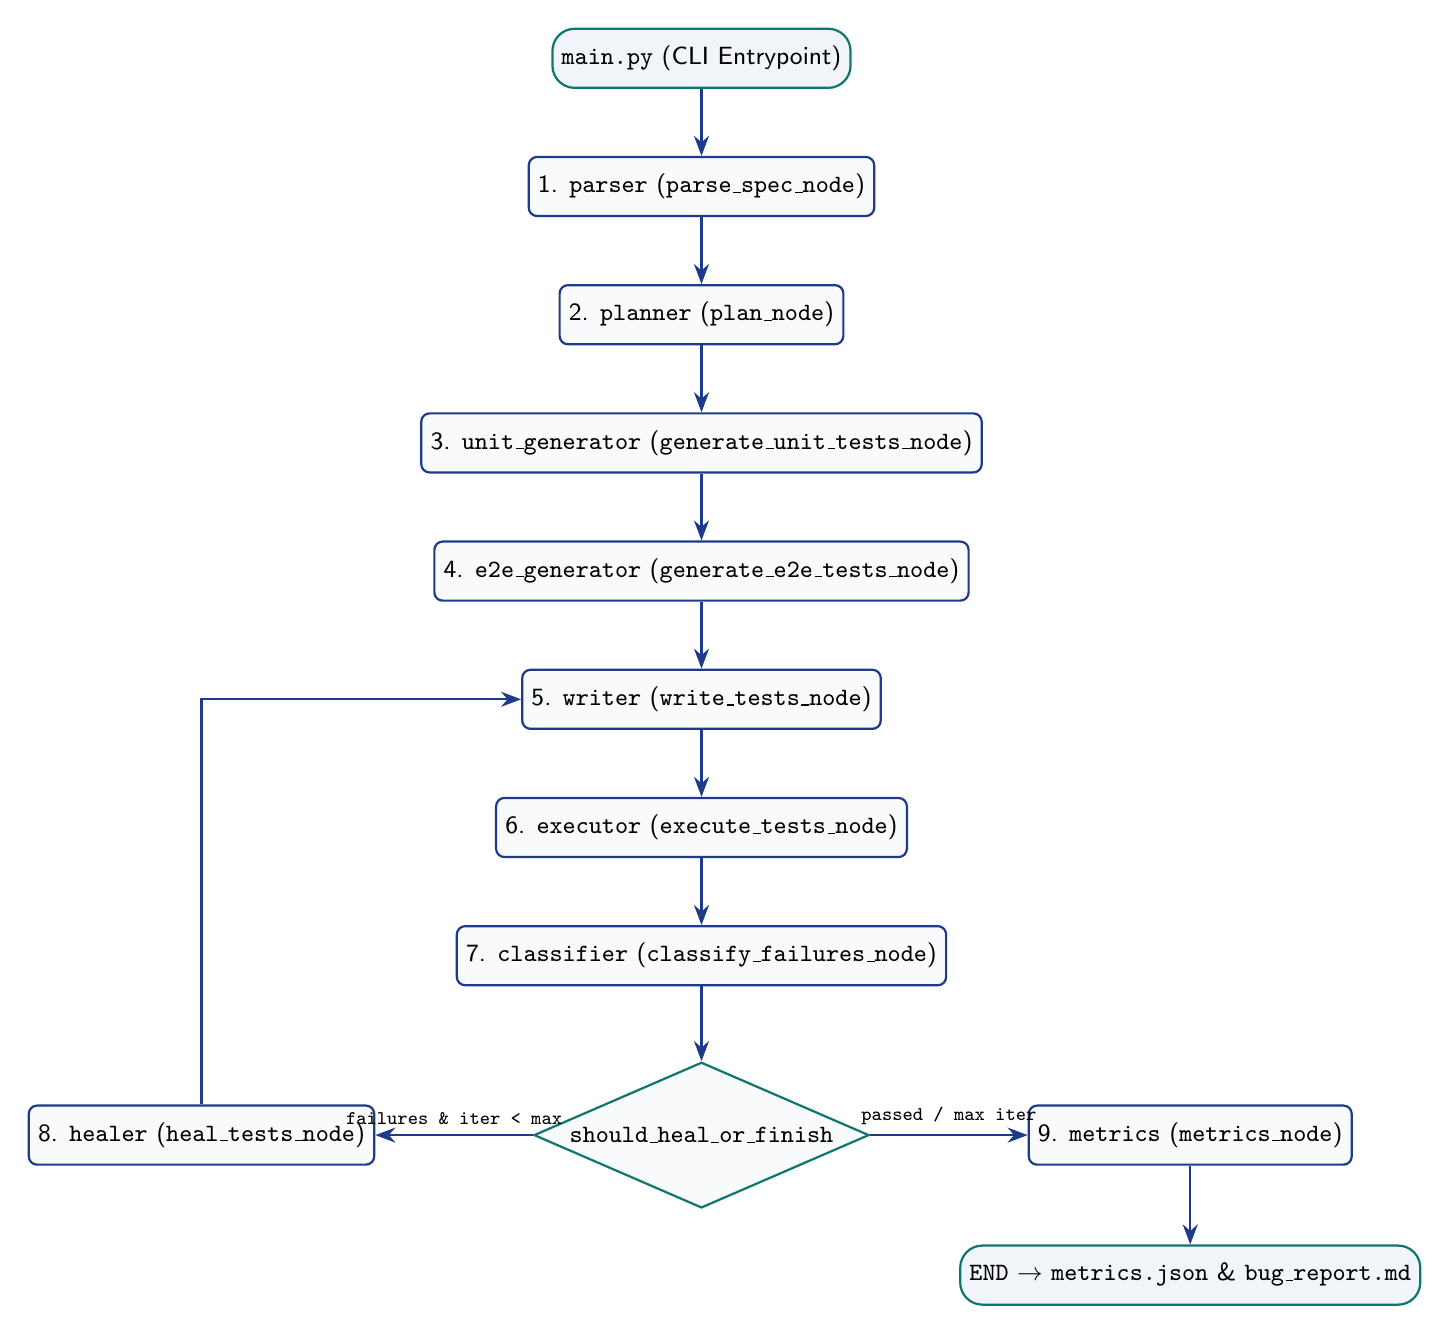
\begin{tikzpicture}[
    node distance=0.85cm and 1.4cm,
    every node/.style={font=\small\sffamily},
    box/.style={rectangle, rounded corners=3pt, draw=PrimaryBlue, fill=LightGray, thick, minimum width=3.4cm, minimum height=0.75cm, align=center},
    decision/.style={diamond, aspect=2.3, draw=AccentTeal, fill=LightGray, thick, align=center, inner sep=2pt},
    term/.style={rectangle, rounded corners=8pt, draw=AccentTeal, fill=CodeBg, thick, minimum width=3.4cm, minimum height=0.75cm, align=center},
    arrow/.style={-{Stealth[scale=1.1]}, thick, draw=PrimaryBlue}
]
    \node[term] (cli) {\texttt{main.py} (CLI Entrypoint)};
    \node[box, below=of cli] (parser) {1. \texttt{parser} (\texttt{parse\_spec\_node})};
    \node[box, below=of parser] (planner) {2. \texttt{planner} (\texttt{plan\_node})};
    \node[box, below=of planner] (unitgen) {3. \texttt{unit\_generator} (\texttt{generate\_unit\_tests\_node})};
    \node[box, below=of unitgen] (e2egen) {4. \texttt{e2e\_generator} (\texttt{generate\_e2e\_tests\_node})};
    \node[box, below=of e2egen] (writer) {5. \texttt{writer} (\texttt{write\_tests\_node})};
    \node[box, below=of writer] (executor) {6. \texttt{executor} (\texttt{execute\_tests\_node})};
    \node[box, below=of executor] (classifier) {7. \texttt{classifier} (\texttt{classify\_failures\_node})};
    \node[decision, below=0.95cm of classifier] (router) {\texttt{should\_heal\_or\_finish}};
    \node[box, left=2.0cm of router] (healer) {8. \texttt{healer} (\texttt{heal\_tests\_node})};
    \node[box, right=2.0cm of router] (metrics) {9. \texttt{metrics} (\texttt{metrics\_node})};
    \node[term, below=1.0cm of metrics] (endnode) {\texttt{END} $\rightarrow$ \texttt{metrics.json} \& \texttt{bug\_report.md}};

    \draw[arrow] (cli) -- (parser);
    \draw[arrow] (parser) -- (planner);
    \draw[arrow] (planner) -- (unitgen);
    \draw[arrow] (unitgen) -- (e2egen);
    \draw[arrow] (e2egen) -- (writer);
    \draw[arrow] (writer) -- (executor);
    \draw[arrow] (executor) -- (classifier);
    \draw[arrow] (classifier) -- (router);
    \draw[arrow] (router) -- node[above, font=\scriptsize]{\texttt{failures \& iter < max}} (healer);
    \draw[arrow] (router) -- node[above, font=\scriptsize]{\texttt{passed / max iter}} (metrics);
    \draw[arrow] (healer.north) |- (writer.west);
    \draw[arrow] (metrics) -- (endnode);
\end{tikzpicture}
\caption{LangGraph \texttt{StateGraph} execution and self-healing loop.}
\label{fig:langgraph_arch}
\end{figure}

% =============================================================================
% SECTION 3: REPOSITORY STRUCTURE
% =============================================================================
\section{Repository Structure}

\begin{lstlisting}
autonomous-api-testing-agent/
|-- benchmark_app/                  # Deliberately buggy FastAPI target (never read by agent)
|   |-- __init__.py                 # Package marker
|   |-- main.py                     # FastAPI CRUD + JWT auth + BUG-1, BUG-2, BUG-3
|   |-- models.py                   # Pydantic v2 schemas with validation constraints
|   `-- Dockerfile.target           # Container image for target_api
|-- docker/
|   |-- Dockerfile.sandbox          # Playwright Chromium + pytest runner container
|   `-- docker-compose.yml          # Isolated test_net bridge network & healthcheck
|-- src/
|   |-- __init__.py                 # Package marker
|   |-- parser/
|   |   |-- __init__.py             # Package marker
|   |   `-- openapi_parser.py       # OpenAPI fetcher, $ref resolver, dep graph, payload gen
|   |-- agent/
|   |   |-- __init__.py             # Package marker
|   |   |-- state.py                # AgentState & TestResult TypedDicts
|   |   |-- prompts.py              # Scoped prompts for local 7B Ollama
|   |   |-- graph.py                # LangGraph StateGraph & conditional routing
|   |   `-- nodes.py                # All 9 node implementations
|   `-- sandbox/
|       |-- __init__.py             # Package marker
|       `-- runner.py               # Docker Compose / local pytest runner & JSON parser
|-- generated_tests/                # Output dir mounted to /tests in Docker
|   |-- .gitkeep
|   |-- conftest.py                 # Session fixtures (client, registered_user, auth_headers)
|   |-- test_unit_endpoints.py      # Seed/generated httpx unit & boundary tests
|   `-- test_e2e_playwright.py      # Seed/generated Playwright E2E + /docs smoke test
|-- reports/
|   `-- .gitkeep                    # Runtime outputs: report.json, metrics.json, bug_report.md
|-- main.py                         # CLI entrypoint
|-- requirements.txt                # Host Python dependencies
|-- README.md                       # Quick-start & high-level overview
|-- DOCUMENTATION.md                # Comprehensive Markdown technical reference
`-- DOCUMENTATION.tex               # This LaTeX technical reference
\end{lstlisting}

% =============================================================================
% SECTION 4: LINE-BY-LINE CODE REFERENCE
% =============================================================================
\section{Line-by-Line Code Reference}

% -----------------------------------------------------------------------------
\subsection{Dependencies: \texttt{requirements.txt}}
% -----------------------------------------------------------------------------
\begin{longtable}{L{1.4cm} L{5.2cm} L{9.0cm}}
\toprule
\textbf{Lines} & \textbf{Content} & \textbf{Purpose} \\
\midrule
\endhead
\texttt{L1} & \texttt{langchain-ollama>=0.2.0} & Provides \texttt{ChatOllama} LangChain wrapper for local Ollama inference. \\
\texttt{L2} & \texttt{langchain-core>=0.3.0} & Core message abstractions (\texttt{SystemMessage}, \texttt{HumanMessage}). \\
\texttt{L3} & \texttt{langgraph>=0.2.0} & Cyclic \texttt{StateGraph} orchestration engine and \texttt{END} sentinel. \\
\texttt{L4} & \texttt{pydantic>=2.0.0} & Schema validation library (v2). \\
\texttt{L5} & \texttt{httpx>=0.27.0} & Synchronous HTTP client used by the OpenAPI parser and generated unit tests. \\
\texttt{L6} & \texttt{docker>=7.0.0} & Docker Python SDK declared alongside \texttt{subprocess} \texttt{docker compose} orchestration. \\
\texttt{L7} & \texttt{pytest>=8.0.0} & Core test runner. \\
\texttt{L8} & \texttt{pytest-playwright>=0.5.0} & Provides \texttt{playwright} and \texttt{page} fixtures for API and Chromium E2E tests. \\
\texttt{L9} & \texttt{pytest-json-report>=1.5.0} & Generates structured \texttt{report.json} with test outcomes and tracebacks. \\
\texttt{L10} & \texttt{ollama>=0.3.0} & Underlying Ollama Python client required by \texttt{langchain-ollama}. \\
\texttt{L11} & \texttt{python-multipart>=0.0.9} & Form-data parsing support (\texttt{OAuth2PasswordRequestForm}). \\
\bottomrule
\end{longtable}

% -----------------------------------------------------------------------------
\subsection{Package Markers \& Placeholders}
% -----------------------------------------------------------------------------
\begin{itemize}[leftmargin=1.5em]
    \item \texttt{benchmark\_app/\_\_init\_\_.py} (empty): Marks \texttt{benchmark\_app} as an importable Python package so \texttt{uvicorn benchmark\_app.main:app} resolves cleanly inside \texttt{Dockerfile.target}.
    \item \texttt{src/\_\_init\_\_.py}, \texttt{src/parser/\_\_init\_\_.py}, \texttt{src/agent/\_\_init\_\_.py}, \texttt{src/sandbox/\_\_init\_\_.py} (empty): Standard Python package markers enabling absolute imports such as \texttt{from src.agent.graph import build\_graph}.
    \item \texttt{generated\_tests/.gitkeep}, \texttt{reports/.gitkeep} (empty): Preserve empty runtime directories in Git prior to test generation and report creation.
\end{itemize}

% -----------------------------------------------------------------------------
\subsection{\texttt{benchmark\_app/models.py}}
% -----------------------------------------------------------------------------
\begin{longtable}{L{1.4cm} L{5.2cm} L{9.0cm}}
\toprule
\textbf{Lines} & \textbf{Code / Construct} & \textbf{Explanation} \\
\midrule
\endhead
\texttt{L1--L2} & \texttt{from pydantic import BaseModel, Field} / \texttt{Optional} & Imports Pydantic v2 base class, field constraint builder, and optional type hint. \\
\texttt{L5--L7} & \texttt{class UserCreate(BaseModel):} & Registration input schema. \texttt{username} requires 3--50 characters (\texttt{min\_length=3, max\_length=50}); \texttt{password} requires at least 6 characters (\texttt{min\_length=6}). Violating either triggers FastAPI HTTP \texttt{422}. \\
\texttt{L10--L12} & \texttt{class UserResponse(BaseModel):} & Public user representation returned after registration (\texttt{id: int}, \texttt{username: str}), intentionally omitting \texttt{password}. \\
\texttt{L15--L17} & \texttt{class Token(BaseModel):} & OAuth2 bearer token response (\texttt{access\_token: str}, \texttt{token\_type: str}). \\
\texttt{L20--L23} & \texttt{class ItemCreate(BaseModel):} & Item creation payload: \texttt{title} (\texttt{1..100} chars), optional \texttt{description}, and \texttt{price} strictly greater than zero (\texttt{gt=0}). \\
\texttt{L26--L29} & \texttt{class ItemUpdate(BaseModel):} & Partial/full update payload where all fields default to \texttt{None} (\texttt{Optional}) while retaining \texttt{min\_length}/\texttt{max\_length}/\texttt{gt=0} constraints when provided. \\
\texttt{L32--L37} & \texttt{class ItemResponse(BaseModel):} & Full item output schema adding server-assigned \texttt{id: int} and \texttt{owner\_id: int}. \\
\bottomrule
\end{longtable}

% -----------------------------------------------------------------------------
\subsection{\texttt{benchmark\_app/main.py}}
% -----------------------------------------------------------------------------
\begin{longtable}{L{1.4cm} L{5.2cm} L{9.0cm}}
\toprule
\textbf{Lines} & \textbf{Code / Construct} & \textbf{Explanation} \\
\midrule
\endhead
\texttt{L1--L4} & Module docstring & Documents the benchmark FastAPI app and notes its 3 intentional defects (\texttt{BUG-1}, \texttt{BUG-2}, \texttt{BUG-3}). \\
\texttt{L6--L21} & Imports & Imports \texttt{datetime}/\texttt{timedelta}, typing generics, FastAPI core classes, \texttt{JSONResponse}/\texttt{Response}, \texttt{OAuth2PasswordBearer}/\texttt{OAuth2PasswordRequestForm}, \texttt{python-jose} (\texttt{JWTError}, \texttt{jwt}), and the 6 Pydantic models from \texttt{benchmark\_app.models}. \\
\texttt{L24--L26} & JWT configuration & Sets \texttt{SECRET\_KEY = "test-secret-key-for-benchmark"}, \texttt{ALGORITHM = "HS256"}, and \texttt{ACCESS\_TOKEN\_EXPIRE\_MINUTES = 60}. \\
\texttt{L29--L32} & In-memory database & Initializes \texttt{users\_db: Dict[str, dict]}, \texttt{items\_db: Dict[int, dict]}, and auto-increment counters \texttt{user\_id\_counter} and \texttt{item\_id\_counter}. \\
\texttt{L35--L41} & \texttt{app = FastAPI(...)} \& \texttt{oauth2\_scheme} & Instantiates FastAPI (automatically serving \texttt{/openapi.json} and \texttt{/docs}) and configures OAuth2 password bearer auth pointing to \texttt{tokenUrl="/auth/token"}. \\
\texttt{L46--L52} & \texttt{\_hash\_password} / \texttt{\_verify\_password} & Simple deterministic \texttt{"hashed:\{password\}"} helper for benchmark isolation. \\
\texttt{L55--L59} & \texttt{\_create\_access\_token} & Copies payload dict, adds UTC \texttt{exp} claim (defaulting to 15 minutes if \texttt{expires\_delta} omitted), and signs HS256 JWT with \texttt{jwt.encode}. \\
\texttt{L62--L80} & \texttt{get\_current\_user} dependency & Extracts Bearer token via \texttt{oauth2\_scheme}, decodes JWT, validates \texttt{sub} claim, looks up \texttt{users\_db[username]}, and raises HTTP \texttt{401 Unauthorized} (\texttt{WWW-Authenticate: Bearer}) on any \texttt{JWTError} or missing user. \\
\texttt{L85--L106} & \texttt{POST /auth/register} & Declares \texttt{201 Created} (\texttt{UserResponse}) and \texttt{422} in OpenAPI. Checks \texttt{users\_db} for duplicate username (raises \texttt{400}), increments \texttt{user\_id\_counter}, stores hashed password, returns \texttt{UserResponse}. \\
\texttt{L109--L127} & \texttt{POST /auth/token} & Accepts form-encoded \texttt{OAuth2PasswordRequestForm}. Validates user existence and password (raises \texttt{401} on mismatch), mints 60-minute JWT with \texttt{"sub": username}, returns \texttt{Token(..., token\_type="bearer")}. \\
\texttt{L132--L156} & \texttt{POST /items/} (\textbf{BUG-3}) & Requires \texttt{get\_current\_user}. Declares \texttt{201 Created} (\texttt{ItemResponse}), \texttt{401}, \texttt{422}. Increments \texttt{item\_id\_counter} and builds \texttt{item} dict. \textbf{Line 152 (\texttt{\# BUG-3}):} hardcodes \texttt{"price": 0.0} instead of \texttt{item\_in.price}, causing the response schema to validate (\texttt{float}) while violating business logic. \\
\texttt{L159--L169} & \texttt{GET /items/} & Authenticated route returning \texttt{[ItemResponse(**item) for item in items\_db.values()]} (\texttt{200 OK}). \\
\texttt{L172--L186} & \texttt{GET /items/\{item\_id\}} (\textbf{BUG-2}) & Authenticated route declaring \texttt{200}, \texttt{401}, and \texttt{404} in OpenAPI. \textbf{Line 185 (\texttt{\# BUG-2}):} directly indexes \texttt{items\_db[item\_id]} without checking membership, raising an unhandled \texttt{KeyError} that FastAPI/Starlette converts into a \texttt{500 Internal Server Error} when \texttt{item\_id} does not exist. \\
\texttt{L189--L214} & \texttt{PUT /items/\{item\_id\}} & Authenticated route declaring \texttt{200}, \texttt{401}, \texttt{404}, \texttt{422}. Correctly raises \texttt{404} if missing; updates only non-\texttt{None} fields from \texttt{ItemUpdate}; saves and returns \texttt{ItemResponse}. \\
\texttt{L217--L235} & \texttt{DELETE /items/\{item\_id\}} (\textbf{BUG-1}) & Authenticated route declaring \texttt{status\_code=204} (\texttt{204}, \texttt{401}, \texttt{404} in OpenAPI). Checks existence (\texttt{404} if absent), deletes from \texttt{items\_db}, then at \textbf{Line 235 (\texttt{\# BUG-1})} returns \texttt{JSONResponse(status\_code=200, content=\{"deleted": True\})}, directly violating its own \texttt{204} OpenAPI contract. \\
\bottomrule
\end{longtable}

% -----------------------------------------------------------------------------
\subsection{\texttt{benchmark\_app/Dockerfile.target}}
% -----------------------------------------------------------------------------
\begin{longtable}{L{1.4cm} L{5.2cm} L{9.0cm}}
\toprule
\textbf{Lines} & \textbf{Instruction} & \textbf{Explanation} \\
\midrule
\endhead
\texttt{L1} & \texttt{FROM python:3.11-slim} & Lightweight Python 3.11 base image. \\
\texttt{L2} & \texttt{WORKDIR /app} & Sets working directory inside the container. \\
\texttt{L3} & \texttt{RUN pip install --no-cache-dir ...} & Installs \texttt{fastapi}, \texttt{uvicorn[standard]}, \texttt{pyjwt}, \texttt{sqlalchemy}, \texttt{pydantic}, \texttt{python-multipart}, and \texttt{python-jose[cryptography]}. \\
\texttt{L4} & \texttt{COPY benchmark\_app/ ./benchmark\_app/} & Copies only the target application package into \texttt{/app/benchmark\_app}. \\
\texttt{L5} & \texttt{EXPOSE 8000} & Documents port \texttt{8000}. \\
\texttt{L6} & \texttt{CMD ["uvicorn", ...]} & Binds Uvicorn to \texttt{0.0.0.0:8000} so \texttt{sandbox\_runner} can reach it over the bridge network. \\
\bottomrule
\end{longtable}

% -----------------------------------------------------------------------------
\subsection{\texttt{docker/Dockerfile.sandbox}}
% -----------------------------------------------------------------------------
\begin{longtable}{L{1.4cm} L{5.2cm} L{9.0cm}}
\toprule
\textbf{Lines} & \textbf{Instruction} & \textbf{Explanation} \\
\midrule
\endhead
\texttt{L1} & \texttt{FROM mcr.microsoft.com/playwright/python:v1.47.0-jammy} & Official Microsoft Playwright Python image pre-bundled with Chromium and system dependencies on Ubuntu Jammy. \\
\texttt{L2} & \texttt{WORKDIR /tests} & Default working directory where generated tests are mounted. \\
\texttt{L3--L9} & \texttt{RUN pip install --no-cache-dir ...} & Installs \texttt{pytest>=8.0.0}, \texttt{httpx>=0.27.0}, \texttt{pytest-playwright>=0.5.0}, \texttt{pytest-json-report>=1.5.0}, \texttt{pytest-xdist>=3.5.0}, and \texttt{lxml}. \\
\texttt{L10} & \texttt{ENV TARGET\_API\_URL=http://target\_api:8000} & Points test fixtures to the \texttt{target\_api} Docker service DNS name. \\
\texttt{L11} & \texttt{CMD ["pytest", "/tests", ...]} & Runs all tests in \texttt{/tests}, emits short tracebacks, writes structured JSON results to \texttt{/reports/report.json}, and ignores any nested \texttt{/tests/reports} directory. \\
\bottomrule
\end{longtable}

% -----------------------------------------------------------------------------
\subsection{\texttt{docker/docker-compose.yml}}
% -----------------------------------------------------------------------------
\begin{longtable}{L{1.4cm} L{5.2cm} L{9.0cm}}
\toprule
\textbf{Lines} & \textbf{Section} & \textbf{Explanation} \\
\midrule
\endhead
\texttt{L1} & \texttt{version: "3.9"} & Compose specification version. \\
\texttt{L3--L18} & \texttt{services.target\_api} & Builds \texttt{benchmark\_app/Dockerfile.target} from parent context \texttt{..}, names container \texttt{target\_api}, exposes host \texttt{8000:8000}, attaches to \texttt{test\_net}, and polls \texttt{http://localhost:8000/openapi.json} every 5s (15 retries, 10s start period) for health. \\
\texttt{L20--L36} & \texttt{services.sandbox\_runner} & Builds \texttt{docker/Dockerfile.sandbox}, waits for \texttt{target\_api} \texttt{condition: service\_healthy}, bind-mounts \texttt{../generated\_tests:/tests} and \texttt{../reports:/reports}, joins \texttt{test\_net}, injects \texttt{TARGET\_API\_URL=http://target\_api:8000}, and uses \texttt{profiles: ["runner"]} so \texttt{docker compose up} does not run tests unless \texttt{--profile runner} is explicitly passed. \\
\texttt{L38--L40} & \texttt{networks.test\_net} & Isolated Docker bridge network connecting \texttt{target\_api} and \texttt{sandbox\_runner}. \\
\bottomrule
\end{longtable}

% -----------------------------------------------------------------------------
\subsection{\texttt{src/parser/openapi\_parser.py}}
% -----------------------------------------------------------------------------
\begin{longtable}{L{1.4cm} L{5.2cm} L{9.0cm}}
\toprule
\textbf{Lines} & \textbf{Construct} & \textbf{Explanation} \\
\midrule
\endhead
\texttt{L1--L10} & Docstring \& imports & Enables \texttt{from \_\_future\_\_ import annotations}, imports \texttt{copy}, \texttt{json}, \texttt{dataclass}/\texttt{field}, typing helpers, and \texttt{httpx}. \\
\texttt{L18--L30} & \texttt{@dataclass class EndpointInfo} & Canonical normalized representation of an API operation: \texttt{path}, \texttt{method}, \texttt{operation\_id}, \texttt{summary}, \texttt{tags}, \texttt{requires\_auth}, \texttt{path\_params}, \texttt{query\_params}, \texttt{request\_body}, \texttt{responses}, and \texttt{success\_status\_code}. \\
\texttt{L38--L52} & \texttt{\_resolve\_ref(ref, root)} & Validates local JSON Pointer (\texttt{\#/}\ldots), splits path tokens, unescapes RFC 6901 tokens (\texttt{\textasciitilde{}1} $\rightarrow$ \texttt{/}, \texttt{\textasciitilde{}0} $\rightarrow$ \texttt{\textasciitilde{}}), and traverses dicts/lists in \texttt{root} to return the referenced node. \\
\texttt{L55--L78} & \texttt{\_resolve\_refs(obj, root, \_visiting)} & Recursively walks dicts and lists. When encountering \texttt{"\$ref"}, checks \texttt{\_visiting} to break cycles (\texttt{\{"\$circular\_ref": ref\_str\}}), adds \texttt{ref\_str} to a new set (\texttt{\_visiting | \{ref\_str\}}), fetches target via \texttt{\_resolve\_ref}, \texttt{copy.deepcopy()}s it so shared definitions stay independent, and recursively resolves nested \texttt{\$ref}s inside it. \\
\texttt{L86--L93} & \texttt{\_scheme\_requires\_auth(scheme)} & Returns \texttt{True} if OpenAPI \texttt{securitySchemes} entry has \texttt{type == "oauth2"} or \texttt{type == "http"} with \texttt{scheme == "bearer"}. \\
\texttt{L96--L111} & \texttt{\_endpoint\_requires\_auth(...)} & Uses operation-level \texttt{security} if present (else falls back to \texttt{global\_security}), checks each requirement object against \texttt{security\_schemes}, and returns \texttt{True} if any scheme is OAuth2 or HTTP Bearer. \\
\texttt{L119--L134} & \texttt{parse\_spec(url)} (fetch \& resolve) & Calls \texttt{httpx.get(url, timeout=30.0)}, raises on HTTP errors, parses JSON, runs \texttt{\_resolve\_refs(raw\_spec, raw\_spec)}, and extracts \texttt{components.securitySchemes} and global \texttt{security}. \\
\texttt{L136--L173} & Path \& parameter extraction & Iterates every path and HTTP method (\texttt{get}, \texttt{post}, \texttt{put}, \texttt{patch}, \texttt{delete}, \texttt{head}, \texttt{options}). Computes \texttt{operation\_id} (falling back to \texttt{\{method\}\_\{sanitized\_path\}}), merges path-level and operation-level parameters keyed by \texttt{(name, in)} so operation-level overrides path-level, and splits into \texttt{path\_params} and \texttt{query\_params}. \\
\texttt{L175--L187} & Request body extraction & Extracts the resolved schema directly from \texttt{requestBody.content}, preferring \texttt{application/json}, then \texttt{application/x-www-form-urlencoded}, then the first available media type. \\
\texttt{L189--L225} & Response \& success-code extraction & Maps each status code in \texttt{responses} to its resolved \texttt{application/json} schema (or \texttt{\{\}} if empty), determines \texttt{success\_status\_code} preferring \texttt{"201"}, \texttt{"200"}, \texttt{"204"} (default \texttt{200}), and appends an \texttt{EndpointInfo}. \\
\texttt{L227--L229} & Deterministic sorting & Sorts endpoints by \texttt{(e.tags[0] if e.tags else "", e.path, e.method)} so test generation order is deterministic across runs. \\
\texttt{L237--L268} & \texttt{build\_dependency\_graph(endpoints)} & Initializes an adjacency dict \texttt{\{operation\_id: []\}}. \texttt{\_resource\_base()} strips trailing \texttt{\{param\}} path segments. Maps \texttt{POST} endpoints without \texttt{path\_params} as resource creators, then adds directed edges \texttt{creator\_id -> ep.operation\_id} for \texttt{GET}/\texttt{PUT}/\texttt{PATCH}/\texttt{DELETE} endpoints that take \texttt{path\_params} on the same resource base. \\
\texttt{L276--L359} & \texttt{generate\_example\_payload(schema)} & Recursively builds minimal valid example values: handles \texttt{allOf}/\texttt{anyOf}/\texttt{oneOf} (first sub-schema), \texttt{"example"}, \texttt{"default"}, \texttt{"enum"}, \texttt{object} (\texttt{properties}), \texttt{array} (\texttt{[item]}), \texttt{string} (honoring \texttt{format} like \texttt{email}/\texttt{date-time}/\texttt{date}/\texttt{uri}, \texttt{minLength}, \texttt{maxLength}), \texttt{number}/\texttt{float} (\texttt{gt}, \texttt{exclusiveMinimum}, \texttt{minimum}), \texttt{integer}, \texttt{boolean}, and \texttt{null}. \\
\texttt{L367--L395} & \texttt{if \_\_name\_\_ == "\_\_main\_\_":} & Standalone diagnostic CLI accepting an optional spec URL (default \texttt{http://localhost:8000/openapi.json}), printing discovered endpoints, auth flags, example payloads, and the dependency graph. \\
\bottomrule
\end{longtable}

% -----------------------------------------------------------------------------
\subsection{\texttt{src/agent/state.py}}
% -----------------------------------------------------------------------------
\begin{longtable}{L{1.4cm} L{5.2cm} L{9.0cm}}
\toprule
\textbf{Lines} & \textbf{Construct} & \textbf{Explanation} \\
\midrule
\endhead
\texttt{L1--L2} & Imports & \texttt{TypedDict}, typing generics, \texttt{Annotated}, and \texttt{operator} (used for list-append reducer). \\
\texttt{L4--L9} & \texttt{class TestResult(TypedDict)} & Schema for each parsed test outcome: \texttt{test\_name}, \texttt{status} (\texttt{passed}/\texttt{failed}/\texttt{error}/\texttt{xfail}), \texttt{failure\_type} (\texttt{TEST\_BUG}/\texttt{API\_BUG}/\texttt{None}), \texttt{traceback}, and \texttt{heal\_action}. \\
\texttt{L11--L38} & \texttt{class AgentState(TypedDict)} & Complete LangGraph shared state across all 9 nodes: \textbf{Inputs} (\texttt{target\_api\_url}, \texttt{openapi\_spec}, \texttt{endpoints}), \textbf{Generation} (\texttt{generated\_unit\_tests}, \texttt{generated\_e2e\_tests}, \texttt{generated\_conftest}), \textbf{Execution \& Healing} (\texttt{iteration}, \texttt{max\_iterations}, \texttt{test\_results}, \texttt{unit\_test\_failures}, \texttt{e2e\_test\_failures}, \texttt{healed\_unit\_tests}, \texttt{healed\_e2e\_tests}), \textbf{Outputs} (\texttt{all\_passed}, \texttt{bug\_reports}, \texttt{metrics}), and \textbf{Control flow} (\texttt{error}, plus \texttt{messages: Annotated[List[str], operator.add]} which instructs LangGraph to append new log entries rather than overwrite previous ones). \\
\bottomrule
\end{longtable}

% -----------------------------------------------------------------------------
\subsection{\texttt{src/agent/prompts.py}}
% -----------------------------------------------------------------------------
\begin{longtable}{L{1.4cm} L{5.2cm} L{9.0cm}}
\toprule
\textbf{Lines} & \textbf{Constant} & \textbf{Explanation} \\
\midrule
\endhead
\texttt{L1--L3} & Module docstring & Explains token-efficiency goal for local \texttt{qwen2.5-coder:7b}. \\
\texttt{L5--L11} & \texttt{UNIT\_TEST\_SYSTEM} & System prompt enforcing \texttt{httpx.Client}, OpenAPI-only testing, coverage of \texttt{200}/\texttt{201}, \texttt{422}, and \texttt{401}, black-box rule, and code-only output. \\
\texttt{L13--L24} & \texttt{UNIT\_TEST\_TEMPLATE} & Per-endpoint prompt injecting \texttt{\{method\}}, \texttt{\{path\}}, \texttt{\{operation\_id\}}, \texttt{\{requires\_auth\}}, \texttt{\{success\_status\_code\}}, \texttt{\{request\_body\}}, \texttt{\{path\_params\}}, \texttt{\{response\_schema\}}, \texttt{\{example\_payload\}}, requesting 3--5 functions using \texttt{client} and \texttt{auth\_headers} fixtures. \\
\texttt{L26--L31} & \texttt{E2E\_SYSTEM} & System prompt for Playwright \texttt{APIRequestContext} stateful journeys ($\text{Register} \rightarrow \text{Login} \rightarrow \text{Create} \rightarrow \text{Mutate} \rightarrow \text{Delete}$) using shared pytest fixtures. \\
\texttt{L33--L44} & \texttt{E2E\_TEMPLATE} & Injects \texttt{\{journey\_name\}}, \texttt{\{steps\}}, \texttt{\{base\_url\}}, \texttt{\{endpoint\_schemas\}} and explicitly requires a Chromium smoke test visiting \texttt{\{base\_url\}/docs} checking \texttt{"Swagger"} in title and visible endpoint blocks. \\
\texttt{L46--L52} & \texttt{HEAL\_SYSTEM} & Self-healing system prompt reinforcing the Black-Box Rule and strict \texttt{TEST\_BUG} vs.\ \texttt{API\_BUG} definitions. \\
\texttt{L54--L71} & \texttt{HEAL\_TEMPLATE} & Provides \texttt{\{original\_test\}}, \texttt{\{traceback\}}, and \texttt{\{endpoint\_spec\}}, lists explicit classification rules, and requests JSON (\texttt{classification}, \texttt{reason}, \texttt{fixed\_code}) followed by the fixed Python function. \\
\texttt{L73--L81} & \texttt{CONFTEST\_TEMPLATE} & Template string describing \texttt{conftest.py} fixtures (retained in \texttt{prompts.py} for reference; \texttt{write\_tests\_node} now renders \texttt{conftest.py} deterministically without an LLM call). \\
\bottomrule
\end{longtable}

% -----------------------------------------------------------------------------
\subsection{\texttt{src/agent/graph.py}}
% -----------------------------------------------------------------------------
\begin{longtable}{L{1.4cm} L{5.2cm} L{9.0cm}}
\toprule
\textbf{Lines} & \textbf{Construct} & \textbf{Explanation} \\
\midrule
\endhead
\texttt{L1--L3} & Imports & \texttt{StateGraph}, \texttt{END}, and \texttt{AgentState}. \\
\texttt{L5--L15} & \texttt{should\_heal\_or\_finish(state)} & Conditional router after \texttt{classifier}: returns \texttt{"metrics"} if \texttt{all\_passed} is True, or if \texttt{iteration >= max\_iterations}, or if no failures exist; otherwise returns \texttt{"healer"} to start another repair cycle. \\
\texttt{L17--L58} & \texttt{build\_graph()} & Imports all 9 node functions from \texttt{src.agent.nodes}, registers nodes (\texttt{parser}, \texttt{planner}, \texttt{unit\_generator}, \texttt{e2e\_generator}, \texttt{writer}, \texttt{executor}, \texttt{classifier}, \texttt{healer}, \texttt{metrics}), sets entry point \texttt{"parser"}, connects linear generation pipeline (\texttt{parser -> planner -> unit\_generator -> e2e\_generator -> writer -> executor -> classifier}), wires conditional edges from \texttt{"classifier"} (\texttt{"healer"} or \texttt{"metrics"}), loops \texttt{"healer" -> "writer"} to persist and re-execute fixes, wires \texttt{"metrics" -> END}, and returns \texttt{graph.compile()}. \\
\bottomrule
\end{longtable}

% -----------------------------------------------------------------------------
\subsection{\texttt{src/agent/nodes.py}}
% -----------------------------------------------------------------------------
\begin{longtable}{L{1.4cm} L{5.2cm} L{9.0cm}}
\toprule
\textbf{Lines} & \textbf{Construct} & \textbf{Explanation} \\
\midrule
\endhead
\texttt{L1--L25} & Imports \& constants & Imports \texttt{os}, \texttt{json}, \texttt{re}, \texttt{Path}, typing helpers, \texttt{ChatOllama}, LangChain messages, \texttt{AgentState}/\texttt{TestResult}, prompts, and parser helpers. Sets \texttt{OLLAMA\_MODEL} (default \texttt{"qwen2.5-coder:7b"}), \texttt{GENERATED\_TESTS\_DIR}, and \texttt{REPORTS\_DIR}. \\
\texttt{L27--L33} & \texttt{get\_llm()} & Instantiates \texttt{ChatOllama} with \texttt{OLLAMA\_MODEL}, \texttt{OLLAMA\_BASE\_URL} (default \texttt{http://localhost:11434}), \texttt{temperature=0.1}, and \texttt{num\_ctx=8192}. \\
\texttt{L35--L41} & \texttt{\_extract\_code\_block(text)} & Regex-extracts code inside \texttt{```python ... ```} fences, falling back to stripped raw text if no fences are present. \\
\texttt{L43--L54} & \texttt{\_extract\_json\_and\_code(text)} & Extracts the first JSON object containing \texttt{"classification"} via regex + \texttt{json.loads()} (safe fallback \texttt{\{\}} on parse error) and extracts the code block via \texttt{\_extract\_code\_block()}. \\
\texttt{L59--L90} & \texttt{parse\_spec\_node(state)} & Calls \texttt{parse\_spec(f"\{url.rstrip('/')\}/openapi.json")}, serializes each \texttt{EndpointInfo} dataclass into plain dicts for LangGraph state compatibility, and handles exceptions by populating \texttt{error} and \texttt{messages}. \\
\texttt{L95--L108} & \texttt{plan\_node(state)} & Formats a human-readable summary of all endpoints (\texttt{METHOD PATH}, \texttt{auth}, \texttt{success}) into \texttt{messages} and initializes \texttt{iteration: 0}. \\
\texttt{L113--L160} & \texttt{generate\_unit\_tests\_node(state)} & Loops through \texttt{endpoints}; if \texttt{request\_body} exists, calls \texttt{generate\_example\_payload(ep["request\_body"])} directly on the resolved schema; formats \texttt{UNIT\_TEST\_TEMPLATE} with character caps; invokes \texttt{llm}; collects extracted functions; prepends \texttt{import pytest} and \texttt{import httpx}; returns \texttt{generated\_unit\_tests}. \\
\texttt{L165--L217} & \texttt{generate\_e2e\_tests\_node(state)} & Builds a compact \texttt{ep\_summary} dict (\texttt{success}, \texttt{auth}, \texttt{body}), defines the 7-step CRUD + post-delete verification journey, formats \texttt{E2E\_TEMPLATE} (capped at 1000 chars), invokes \texttt{llm}, prepends standard imports (\texttt{pytest}, \texttt{uuid}, \texttt{APIRequestContext}, \texttt{Page}), and returns \texttt{generated\_e2e\_tests}. \\
\texttt{L222--L278} & \texttt{write\_tests\_node(state)} & Creates \texttt{generated\_tests/} and \texttt{reports/}, renders a deterministic \texttt{conftest.py} (with \texttt{base\_url}, \texttt{client}, \texttt{unique\_username}, \texttt{registered\_user}, \texttt{auth\_token}, \texttt{auth\_headers}, \texttt{playwright\_base\_url}), selects \texttt{healed\_unit\_tests}/\texttt{healed\_e2e\_tests} if present (else initial generated tests), and writes \texttt{conftest.py}, \texttt{test\_unit\_endpoints.py}, and \texttt{test\_e2e\_playwright.py} to disk. \\
\texttt{L283--L301} & \texttt{execute\_tests\_node(state)} & Reads \texttt{SANDBOX\_MODE} env var (default \texttt{"docker"}), calls \texttt{run\_tests\_in\_sandbox(mode=mode)}, and updates \texttt{test\_results}, \texttt{unit\_test\_failures}, \texttt{e2e\_test\_failures}, \texttt{all\_passed}, and \texttt{messages}. \\
\texttt{L306--L382} & \texttt{classify\_failures\_node(state)} & Combines unit + E2E failures; if empty, returns immediately. Otherwise loops over each failure, matches the corresponding endpoint spec by path/\texttt{operation\_id} substring, invokes \texttt{llm} with \texttt{HEAL\_SYSTEM} + \texttt{HEAL\_TEMPLATE}, parses \texttt{classification} (\texttt{TEST\_BUG} default) / \texttt{reason} / \texttt{fixed\_code}, appends \texttt{API\_BUG} entries using \texttt{relevant\_ep["path"]} into \texttt{bug\_reports}, and splits failures back into \texttt{unit\_test\_failures} and \texttt{e2e\_test\_failures}. \\
\texttt{L387--L436} & \texttt{heal\_tests\_node(state)} & Loads current unit \& E2E test strings. \texttt{apply\_fixes()} iterates failures: for \texttt{API\_BUG}, prepends \texttt{@pytest.mark.xfail(reason="API\_BUG: ...", strict=True)} above \texttt{def \{test\_name\}(}; for \texttt{TEST\_BUG}, regex-replaces the failing \texttt{def \{test\_name\}(...):...} block with \texttt{fixed\_code}. Increments \texttt{iteration} and stores \texttt{healed\_unit\_tests} / \texttt{healed\_e2e\_tests}. \\
\texttt{L441--L517} & \texttt{metrics\_node(state)} & Tallies \texttt{total}, \texttt{passed}, \texttt{failed}, \texttt{xfailed}, computes \texttt{zero\_shot\_pass\_rate} and \texttt{post\_healing\_pass\_rate}, writes \texttt{reports/metrics.json}, and builds/writes \texttt{reports/bug\_report.md} listing each detected API bug with endpoint, test name, reason, and 500-char traceback excerpt. \\
\bottomrule
\end{longtable}

% -----------------------------------------------------------------------------
\subsection{\texttt{src/sandbox/runner.py}}
% -----------------------------------------------------------------------------
\begin{longtable}{L{1.4cm} L{5.2cm} L{9.0cm}}
\toprule
\textbf{Lines} & \textbf{Construct} & \textbf{Explanation} \\
\midrule
\endhead
\texttt{L1--L17} & Docstring, imports \& paths & Imports \texttt{os}, \texttt{json}, \texttt{subprocess}, \texttt{tempfile}, \texttt{xml.etree.ElementTree}, \texttt{Path}, typing. Defines \texttt{GENERATED\_TESTS\_DIR}, \texttt{REPORTS\_DIR}, and \texttt{DOCKER\_COMPOSE\_FILE}. \\
\texttt{L19--L38} & \texttt{run\_tests\_in\_sandbox(mode, timeout)} & Dispatches to \texttt{\_run\_docker()} if \texttt{mode == "docker"} and \texttt{\_docker\_available()}, else falls back to \texttt{\_run\_local()}. \\
\texttt{L40--L47} & \texttt{\_docker\_available()} & Runs \texttt{docker info} with 5s timeout; returns \texttt{True} if exit code is \texttt{0}. \\
\texttt{L49--L88} & \texttt{\_run\_docker(timeout)} & Ensures \texttt{reports/} exists, builds compose images (\texttt{docker compose -f docker/docker-compose.yml build}), returns \texttt{\_error\_result} if build fails, runs \texttt{--profile runner up --abort-on-container-exit --exit-code-from sandbox\_runner}, and parses \texttt{reports/report.json} (falling back to \texttt{\_parse\_pytest\_output} if missing). \\
\texttt{L90--L115} & \texttt{\_run\_local(timeout)} & Runs \texttt{pytest generated\_tests --tb=short --json-report --json-report-file=reports/report.json -v --ignore generated\_tests/reports} locally and parses \texttt{report.json} or stdout fallback. \\
\texttt{L117--L182} & \texttt{\_parse\_json\_report(report\_path, raw\_output)} & Reads \texttt{report.json}, extracts summary counts (\texttt{passed}, \texttt{failed}, \texttt{error}), maps pytest outcomes (\texttt{xfailed} $\rightarrow$ \texttt{xfail}, \texttt{xpassed} $\rightarrow$ \texttt{xpass}, etc.), truncates \texttt{call.longrepr} tracebacks to 2000 chars, fetches function source via \texttt{\_get\_test\_source()}, separates failures into \texttt{e2e\_failures} (nodeid contains \texttt{"playwright"} or \texttt{"e2e"}) vs.\ \texttt{unit\_failures}, and returns normalized dict. \\
\texttt{L184--L211} & \texttt{\_parse\_pytest\_output(raw\_output)} & Regex fallback parsing \texttt{(\textbackslash d+) passed}, \texttt{(\textbackslash d+) failed}, \texttt{(\textbackslash d+) error} from pytest summary line when JSON report is unavailable. \\
\texttt{L213--L232} & \texttt{\_get\_test\_source(nodeid)} & Resolves file path inside \texttt{generated\_tests/} from pytest \texttt{nodeid} and regex-extracts up to 1000 chars of the target \texttt{def func\_name(...)} for healing context. \\
\texttt{L234--L244} & \texttt{\_error\_result(msg)} & Constructs a failure payload under \texttt{"sandbox\_startup"} when Docker build or startup fails. \\
\bottomrule
\end{longtable}

% -----------------------------------------------------------------------------
\subsection{\texttt{main.py}}
% -----------------------------------------------------------------------------
\begin{longtable}{L{1.4cm} L{5.2cm} L{9.0cm}}
\toprule
\textbf{Lines} & \textbf{Construct} & \textbf{Explanation} \\
\midrule
\endhead
\texttt{L1--L14} & Shebang, docstring \& imports & Standard CLI docstring with examples; imports \texttt{argparse}, \texttt{json}, \texttt{os}, \texttt{sys}, \texttt{Path}. \\
\texttt{L16--L53} & \texttt{parse\_args()} & Defines \texttt{--url} (\texttt{http://localhost:8000}), \texttt{--model} (\texttt{qwen2.5-coder:7b}), \texttt{--iterations} (\texttt{3}), \texttt{--local} (flag), \texttt{--skip-e2e} (flag), and \texttt{--ollama-url} (\texttt{http://localhost:11434}). \\
\texttt{L55--L77} & \texttt{main()} setup & Exports \texttt{OLLAMA\_MODEL}, \texttt{OLLAMA\_BASE\_URL}, and \texttt{SANDBOX\_MODE="local"} (if \texttt{--local} set) before importing \texttt{build\_graph()} so module-level env defaults pick up CLI values. Prints startup banner and compiles graph. \\
\texttt{L78--L108} & \texttt{initial\_state} \& streaming & Seeds all \texttt{AgentState} keys and streams \texttt{graph.stream(initial\_state, stream\_mode="values")}, printing the latest \texttt{messages[-1]} line as each node finishes. \\
\texttt{L110--L154} & Reporting \& exit codes & Exits \texttt{1} if \texttt{final\_state} missing or \texttt{error} set. Prints formatted summary box (\texttt{total\_tests}, \texttt{passed}, \texttt{failed}, \texttt{xfailed\_api\_bugs}, pass rates, \texttt{healing\_iterations}, \texttt{bug\_reports}), lists detected API bugs, and exits \texttt{2} if any unhealed \texttt{TEST\_BUG} failures remain after \texttt{max\_iterations}. \\
\texttt{L156--L157} & Entrypoint guard & Calls \texttt{main()} under \texttt{if \_\_name\_\_ == "\_\_main\_\_":}. \\
\bottomrule
\end{longtable}

% -----------------------------------------------------------------------------
\subsection{\texttt{generated\_tests/conftest.py}}
% -----------------------------------------------------------------------------
Seed/template fixture file (overwritten at runtime by \texttt{write\_tests\_node}):
\begin{longtable}{L{1.4cm} L{5.2cm} L{9.0cm}}
\toprule
\textbf{Lines} & \textbf{Fixture / Code} & \textbf{Explanation} \\
\midrule
\endhead
\texttt{L1--L9} & Docstring, imports \& default URL & Imports \texttt{uuid}, \texttt{pytest}, \texttt{httpx}; defines fallback \texttt{TARGET\_API\_URL = "http://localhost:8000"}. \\
\texttt{L11--L14} & \texttt{base\_url} (session) & Reads \texttt{TARGET\_API\_URL} env var so Docker runs automatically hit \texttt{http://target\_api:8000}. \\
\texttt{L16--L19} & \texttt{client} (session) & Yields a persistent \texttt{httpx.Client(base\_url=base\_url, timeout=10.0)} and closes it cleanly on teardown. \\
\texttt{L21--L23} & \texttt{unique\_username} (session) & Generates \texttt{testuser\_<8-hex-chars>} per session. \\
\texttt{L25--L33} & \texttt{registered\_user} (session) & Sends \texttt{POST /auth/register}, asserts \texttt{201}, returns credentials dict. \\
\texttt{L35--L49} & \texttt{auth\_token} (session) & Sends \texttt{POST /auth/token} with \texttt{application/x-www-form-urlencoded} form data, asserts \texttt{200}, returns \texttt{access\_token}. \\
\texttt{L51--L54} & \texttt{auth\_headers} (session) & Returns \texttt{\{"Authorization": f"Bearer \{auth\_token\}"\}}. \\
\texttt{L56--L58} & \texttt{playwright\_base\_url} (session) & Aliases \texttt{base\_url} for Playwright tests. \\
\bottomrule
\end{longtable}

% -----------------------------------------------------------------------------
\subsection{\texttt{generated\_tests/test\_unit\_endpoints.py}}
% -----------------------------------------------------------------------------
Seed unit test suite covering 15 test cases across all endpoints:
\begin{longtable}{L{1.4cm} L{5.2cm} L{9.0cm}}
\toprule
\textbf{Lines} & \textbf{Section / Tests} & \textbf{Explanation} \\
\midrule
\endhead
\texttt{L1--L7} & Docstring \& imports & Imports \texttt{pytest} and \texttt{httpx} and documents Black-Box Rule. \\
\texttt{L13--L49} & \texttt{POST /auth/register} & \texttt{test\_register\_happy\_path} (\texttt{201}), \texttt{test\_register\_username\_too\_short} (\texttt{422} for 2 chars), \texttt{test\_register\_password\_too\_short} (\texttt{422} for 5 chars), \texttt{test\_register\_duplicate\_username} (\texttt{400}/\texttt{409}). \\
\texttt{L55--L74} & \texttt{POST /auth/token} & \texttt{test\_login\_happy\_path} (\texttt{200} + \texttt{access\_token} + \texttt{"bearer"}), \texttt{test\_login\_wrong\_password} (\texttt{401}). \\
\texttt{L80--L115} & \texttt{POST /items/} & \texttt{test\_create\_item\_happy\_path} (\texttt{201}), \texttt{test\_create\_item\_no\_auth} (\texttt{401}), \texttt{test\_create\_item\_invalid\_price} (\texttt{422} for \texttt{-1.0}), \texttt{test\_create\_item\_title\_empty} (\texttt{422} for \texttt{""}). \\
\texttt{L121--L130} & \texttt{GET /items/} & \texttt{test\_list\_items\_happy\_path} (\texttt{200} + \texttt{list}), \texttt{test\_list\_items\_no\_auth} (\texttt{401}). \\
\texttt{L136--L145} & \texttt{GET /items/\{item\_id\}} & \texttt{test\_get\_item\_not\_found} (expects \texttt{404}; triggers \textbf{BUG-2} \texttt{500} on benchmark app), \texttt{test\_get\_item\_no\_auth} (\texttt{401}). \\
\texttt{L151--L154} & \texttt{DELETE /items/\{item\_id\}} & \texttt{test\_delete\_item\_no\_auth} (\texttt{401}). \\
\bottomrule
\end{longtable}

% -----------------------------------------------------------------------------
\subsection{\texttt{generated\_tests/test\_e2e\_playwright.py}}
% -----------------------------------------------------------------------------
Seed Playwright E2E + UI smoke test suite:
\begin{longtable}{L{1.4cm} L{5.2cm} L{9.0cm}}
\toprule
\textbf{Lines} & \textbf{Construct / Tests} & \textbf{Explanation} \\
\midrule
\endhead
\texttt{L1--L9} & Docstring \& imports & Imports \texttt{json}, \texttt{uuid}, \texttt{pytest}, \texttt{APIRequestContext}, \texttt{Page}, \texttt{Playwright}. \\
\texttt{L12--L20} & \texttt{api\_request\_context} fixture & Session-scoped fixture creating \texttt{playwright.request.new\_context(base\_url=playwright\_base\_url, extra\_http\_headers=\{"Content-Type": "application/json"\})} and disposing it on teardown. \\
\texttt{L23--L29} & \texttt{TestFullUserJourney} \& \texttt{journey\_state} & Test class grouping sequential journey steps sharing a class-scoped \texttt{journey\_state} dictionary. \\
\texttt{L31--L44} & \texttt{test\_01\_register} & \texttt{POST /auth/register}, asserts \texttt{201}, stores \texttt{username}, \texttt{password}, \texttt{user\_id}. \\
\texttt{L46--L58} & \texttt{test\_02\_login} & \texttt{POST /auth/token} using Playwright \texttt{form=\{...\}}, asserts \texttt{200}, stores \texttt{token}. \\
\texttt{L60--L72} & \texttt{test\_03\_create\_item} & \texttt{POST /items/} with \texttt{Bearer} header, asserts \texttt{201}, stores \texttt{item\_id} (notes \textbf{BUG-3}). \\
\texttt{L74--L81} & \texttt{test\_04\_get\_item} & \texttt{GET /items/\{item\_id\}}, asserts \texttt{200} and matching \texttt{id}. \\
\texttt{L83--L94} & \texttt{test\_05\_update\_item} & \texttt{PUT /items/\{item\_id\}}, asserts \texttt{200} and updated \texttt{title}. \\
\texttt{L96--L103} & \texttt{test\_06\_delete\_item} & \texttt{DELETE /items/\{item\_id\}}, asserts \texttt{204} (catches \textbf{BUG-1} returning \texttt{200}). \\
\texttt{L105--L114} & \texttt{test\_07\_get\_deleted\_item} & \texttt{GET /items/\{item\_id\}} after delete, asserts \texttt{404} (catches \textbf{BUG-2} returning \texttt{500}). \\
\texttt{L117--L136} & \texttt{TestSwaggerUISmokeTest.test\_swagger\_ui\_loads} & Navigates headless Chromium \texttt{Page} to \texttt{\{playwright\_base\_url\}/docs}, waits for \texttt{networkidle}, asserts \texttt{"swagger"} in \texttt{page.title().lower()}, asserts \texttt{.opblock} count $> 0$, and asserts \texttt{"/items"} appears in rendered HTML. \\
\bottomrule
\end{longtable}

% -----------------------------------------------------------------------------
\subsection{\texttt{README.md}}
% -----------------------------------------------------------------------------
\begin{itemize}[leftmargin=1.5em]
    \item \texttt{L1--L389}: High-level user guide covering architecture overview, tech stack, hardware/software prerequisites, quick-start steps, deliberate bugs table, configuration, outputs, and extension guide.
    \item \textbf{Documentation Note:} \texttt{README.md} retains a few stale placeholder names from initial generation (referencing \texttt{python -m agent.main}, \texttt{codellama:7b}, and \texttt{agent/nodes/} instead of the actual entrypoint \texttt{python main.py}, default model \texttt{qwen2.5-coder:7b}, and \texttt{src/agent/} package layout). Treat \texttt{DOCUMENTATION.md}, this LaTeX reference, and \texttt{main.py} as authoritative.
\end{itemize}

% =============================================================================
% SECTION 5: VERIFICATION FIXES & ENGINEERING OBSERVATIONS
% =============================================================================
\section{Verification Fixes \& Engineering Observations}

\subsection{Fixes Applied During Verification}
\begin{enumerate}[leftmargin=1.5em]
    \item \textbf{\texttt{SANDBOX\_MODE} propagation (\texttt{src/agent/nodes.py}):} \texttt{execute\_tests\_node} originally called \texttt{run\_tests\_in\_sandbox()} with no arguments, ignoring \texttt{--local}. Updated to read \texttt{os.getenv("SANDBOX\_MODE", "docker")} and pass \texttt{mode=mode}.
    \item \textbf{Loop variable shadowing (\texttt{src/agent/nodes.py}):} \texttt{classify\_failures\_node} referenced \texttt{ep["path"]} instead of \texttt{relevant\_ep["path"]} when recording \texttt{api\_bugs}, risking wrong endpoint attribution or \texttt{NameError}. Fixed to \texttt{relevant\_ep["path"]}.
    \item \textbf{Deterministic \texttt{conftest.py} (\texttt{src/agent/nodes.py}):} \texttt{write\_tests\_node} previously spent an Ollama LLM call on every healing loop to regenerate \texttt{conftest.py}. Replaced with a deterministic template string.
    \item \textbf{Schema double-extraction (\texttt{src/agent/nodes.py}):} \texttt{generate\_unit\_tests\_node} previously looked up \texttt{ep["request\_body"]["content"]["application/json"]["schema"]}, whereas \texttt{openapi\_parser.py} already stores the unwrapped schema directly under \texttt{ep["request\_body"]}. Fixed to call \texttt{generate\_example\_payload(ep["request\_body"])}.
    \item \textbf{OpenAPI \texttt{204} contract declaration (\texttt{benchmark\_app/main.py}):} \texttt{delete\_item} previously declared \texttt{200} in its \texttt{@app.delete(..., responses=\{...\})} decorator, masking \textbf{BUG-1} from black-box tests. Updated to declare \texttt{status\_code=204} in OpenAPI while keeping \texttt{JSONResponse(status\_code=200, ...)} in the handler body so \textbf{BUG-1} is a genuine spec violation.
\end{enumerate}

\subsection{Remaining Implementation Notes for Future Hardening}
\begin{calloutbox}[WarnAmber]{Engineering Hardening Notes}
\begin{itemize}[leftmargin=1.5em]
    \item \textbf{\texttt{--skip-e2e} flag (\texttt{main.py}):} \texttt{parse\_args()} accepts \texttt{--skip-e2e}, though \texttt{main()} does not yet forward it into \texttt{AgentState} or bypass \texttt{generate\_e2e\_tests\_node}.
    \item \textbf{\texttt{zero\_shot\_pass\_rate} tracking (\texttt{src/agent/nodes.py}):} \texttt{metrics\_node} filters \texttt{[r for r in test\_results if r.get("iteration", 0) == 0]}. Because \texttt{runner.py} does not tag \texttt{"iteration"} onto individual \texttt{TestResult} items, \texttt{r.get("iteration", 0)} defaults to \texttt{0} on every iteration, meaning multi-iteration runs compute \texttt{zero\_shot\_pass\_rate} from the final run unless iteration \texttt{0} results are snapshotted separately.
    \item \textbf{Host vs.\ Container \texttt{TARGET\_API\_URL}:} In Docker mode (\texttt{python main.py --url http://localhost:8000}), \texttt{parse\_spec\_node} fetches \texttt{http://localhost:8000/openapi.json} from the host, while \texttt{write\_tests\_node} embeds \texttt{os.getenv("TARGET\_API\_URL", base\_url)} into \texttt{conftest.py}, which \texttt{docker-compose.yml} overrides to \texttt{http://target\_api:8000} inside \texttt{sandbox\_runner}.
\end{itemize}
\end{calloutbox}

\end{document}

